77. $\cfrac{(x^2-7x+10)(x^2-8x+16)}{\sqrt{x+10}(-2x^2+3x-10)}\leqslant 0\Leftrightarrow \cfrac{(x-5)(x-2)(x-4)^2}{\sqrt{x+10}(x^2+(x-1,5)^2+7,75)}\geqslant 0.$
Применив метод интервалов, найдём ответ: $x\in(-10;2]\cup\{4\}\cup[5;+\infty).$
\begin{figure}[ht!]
\center{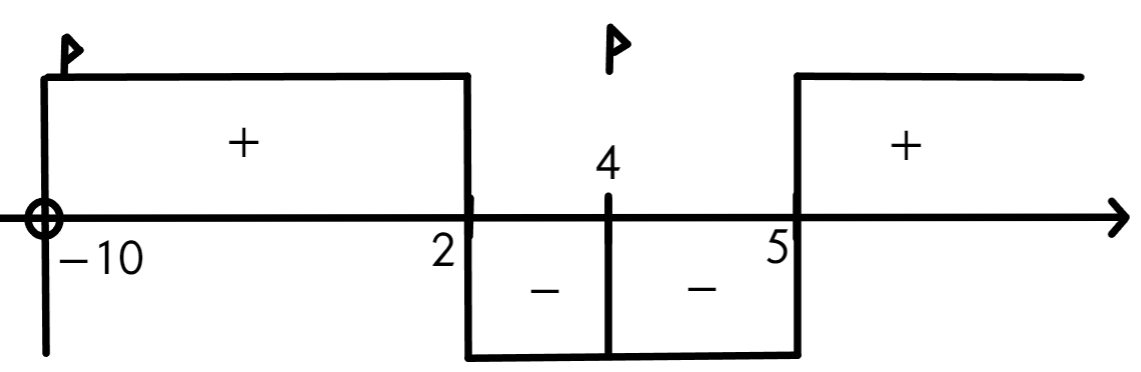
\includegraphics[scale=0.35]{ner9-77.png}}
\end{figure}\\
